\section{Climate Policy and Implications}
\label{sec:climate_policy}

It is clear that there is an anthropogenic impac on the climate as per all of the
information presented in the previous sections. The question now is what can be done
about it such that humanity can continue to enjoy prosperity.\\

Precisely because anthropogenic climate change is believed to be a threat to said
prosperity, there has been international recognition of the need to implement 
policies to mitigate the effects and the scale of dangerous climate change. The 
most clear example of this is the 2015 Paris Agreement, which was signed by 200
countries and sets out the following goals:
\begin{itemize}
    \item To limit the increase in global surface temperature by \textless{}2K above 
    pre-industrial revolution levels by the end of 2100.
    \item To achieve ``net-zero'' emissions by the second half of the 21st century,
    allowing for carbon capture technology to be used to offset any remaining
    emissions.
    \item To set up a ``global stocktake'' to assess whether the goals are being
    met by individual countries. This is also called the \textbf{intended nationally
    determined contributions} (INDCs). The first such stocktake will be in 2023.
\end{itemize}

The Paris Agreement is complementary to the UN's 17 Sustainable Development Goals
(SDGs), which are a set of goals to be achieved by 2030. See Figure \ref{fig:SDGs}.

\begin{figure}[ht]
    \centering
    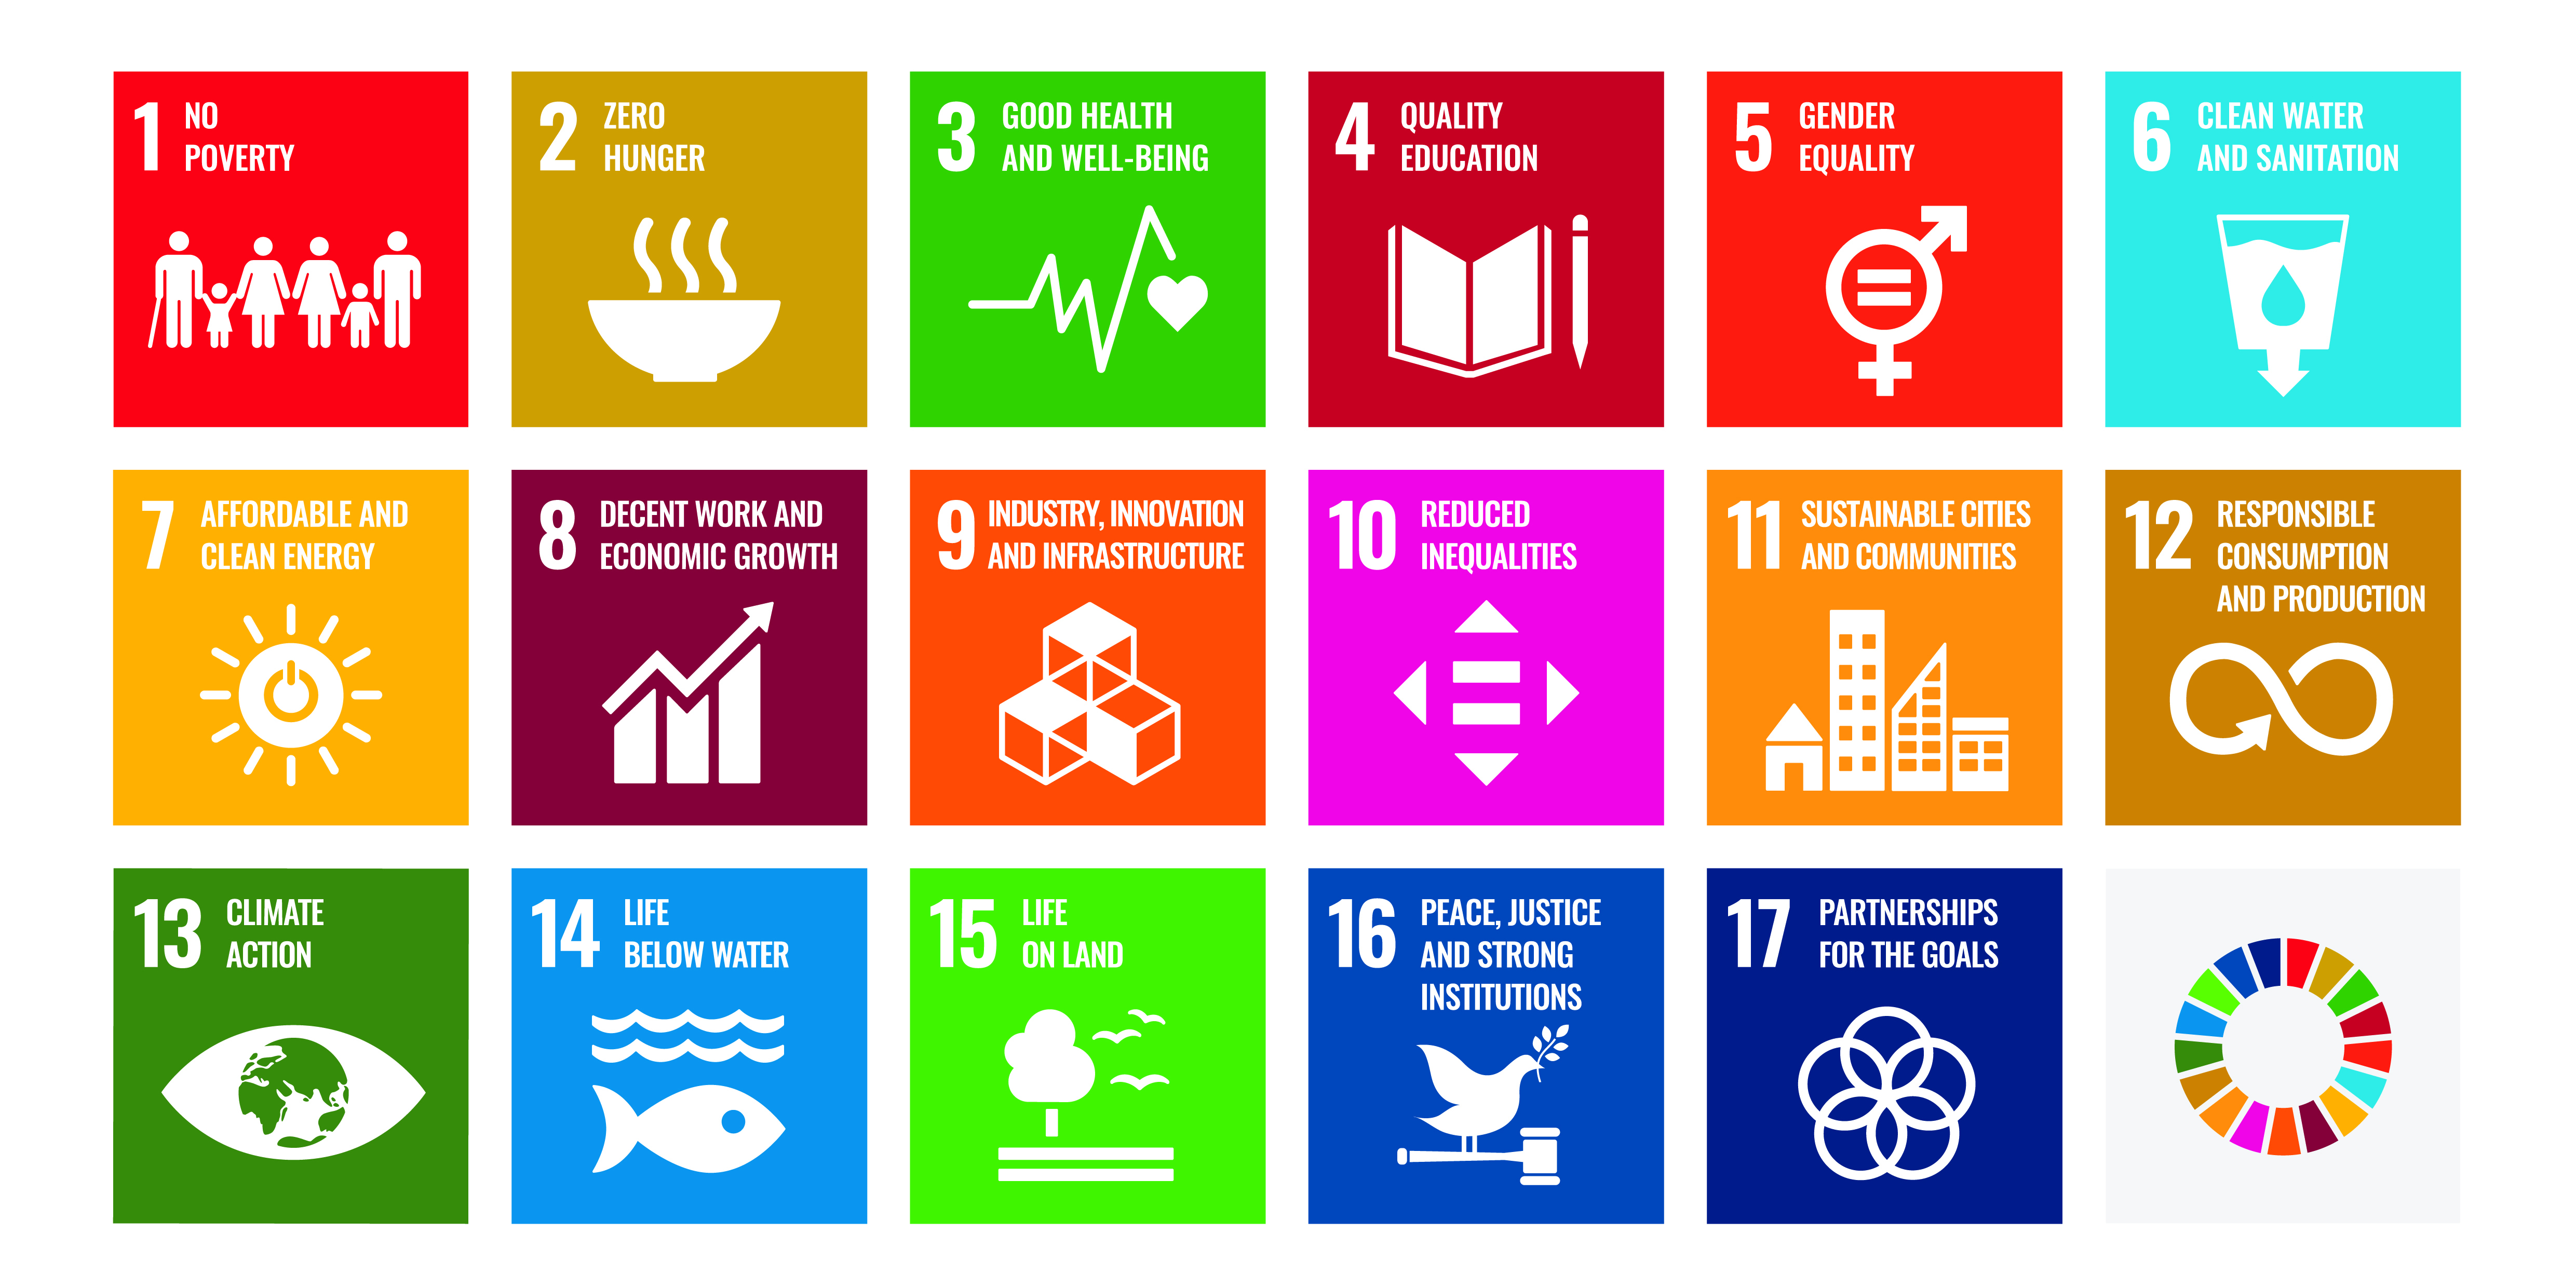
\includegraphics[width=0.85\textwidth]{figures/sdg.jpeg}
    \caption{The 17 Sustainable Development Goals}
    \label{fig:SDGs}
\end{figure}

\subsection{How to Achieve the Climate Goals}
\label{sec:achieve_climate_goals}

The above goals are ambitious, so if we wish to achieve them we have to analyse
what the existing patterns of emissions are and how they need to be changed to
achieve the goals.

\begin{figure}[ht]
    \centering
    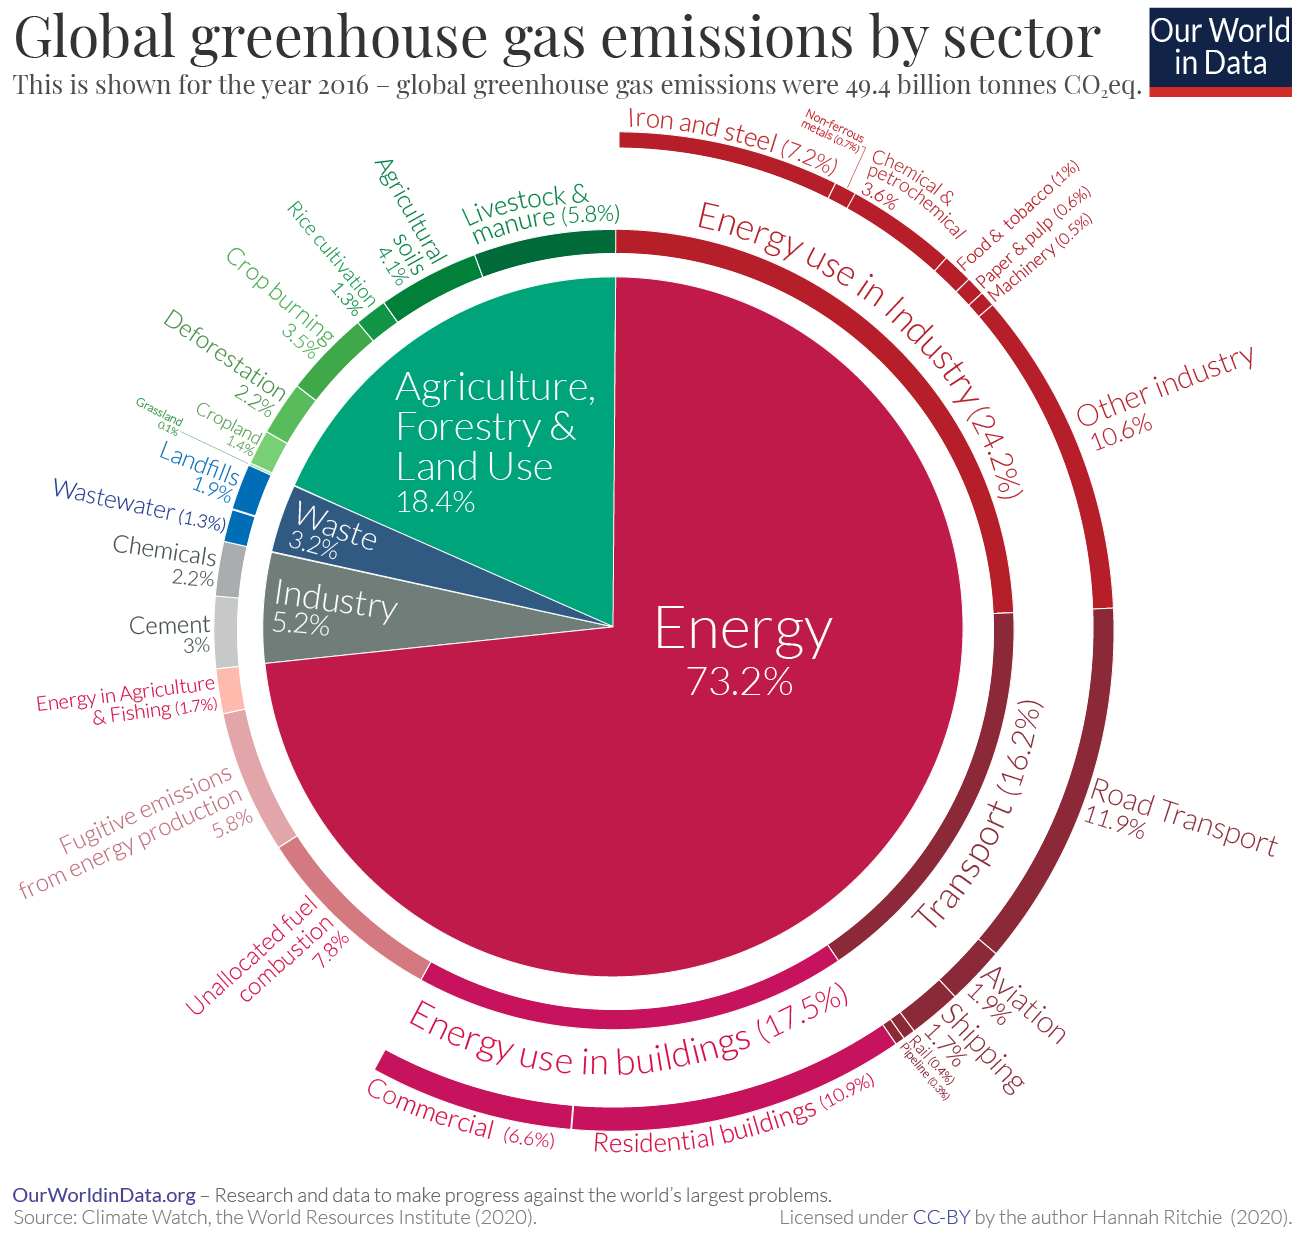
\includegraphics[width=0.55\textwidth]{figures/emissions-pie-chart.png}
    \caption{Global \ce{CO2} emissions by sector}
    \label{fig:emissions_pie_chart}
\end{figure}

Figure \ref{fig:emissions_pie_chart} shows us the breakdown of global \ce{CO2}
emissions by sector. We clearly see that if we wish to limit the anthropogenic
impact of climate change, we need to focus on the energy sector. \\

\noindent The \textbf{Kaya Identity} allows us to relate the total emissions to four key
factors: population, GDP per capita, energy intensity and carbon intensity:
\begin{equation*}
    \boxed{
    \begin{array}{c c c c c c c c c}
    \text{Total Emissions} & = & \text{Population} & \times & \text{GDP per capita}
    & \times & \text{Energy Intensity} & \times & \text{Carbon Intensity} \\
    \text{F\ (kg)} & = & \text{P} & \times & \text{GDPP (\$ pp)} &\times & \text{EI\ (kWh/\$)}
    & \times & \text{CI\ (kg/kWh)}\\
    \end{array}}
\end{equation*}

We see that in the past decades the increase in emissions (F) is largely due to 
the population increase as well as the increase in GDP per capita. By contrast, 
the energy intensity and carbon intensity have decreased, though to a smaller
extent. See Figure \ref{fig:kaya_components}. We also note that these individual
factors change from country to country (for more details see L12 slides 9 onwards).

\begin{figure}[ht]
    \centering
    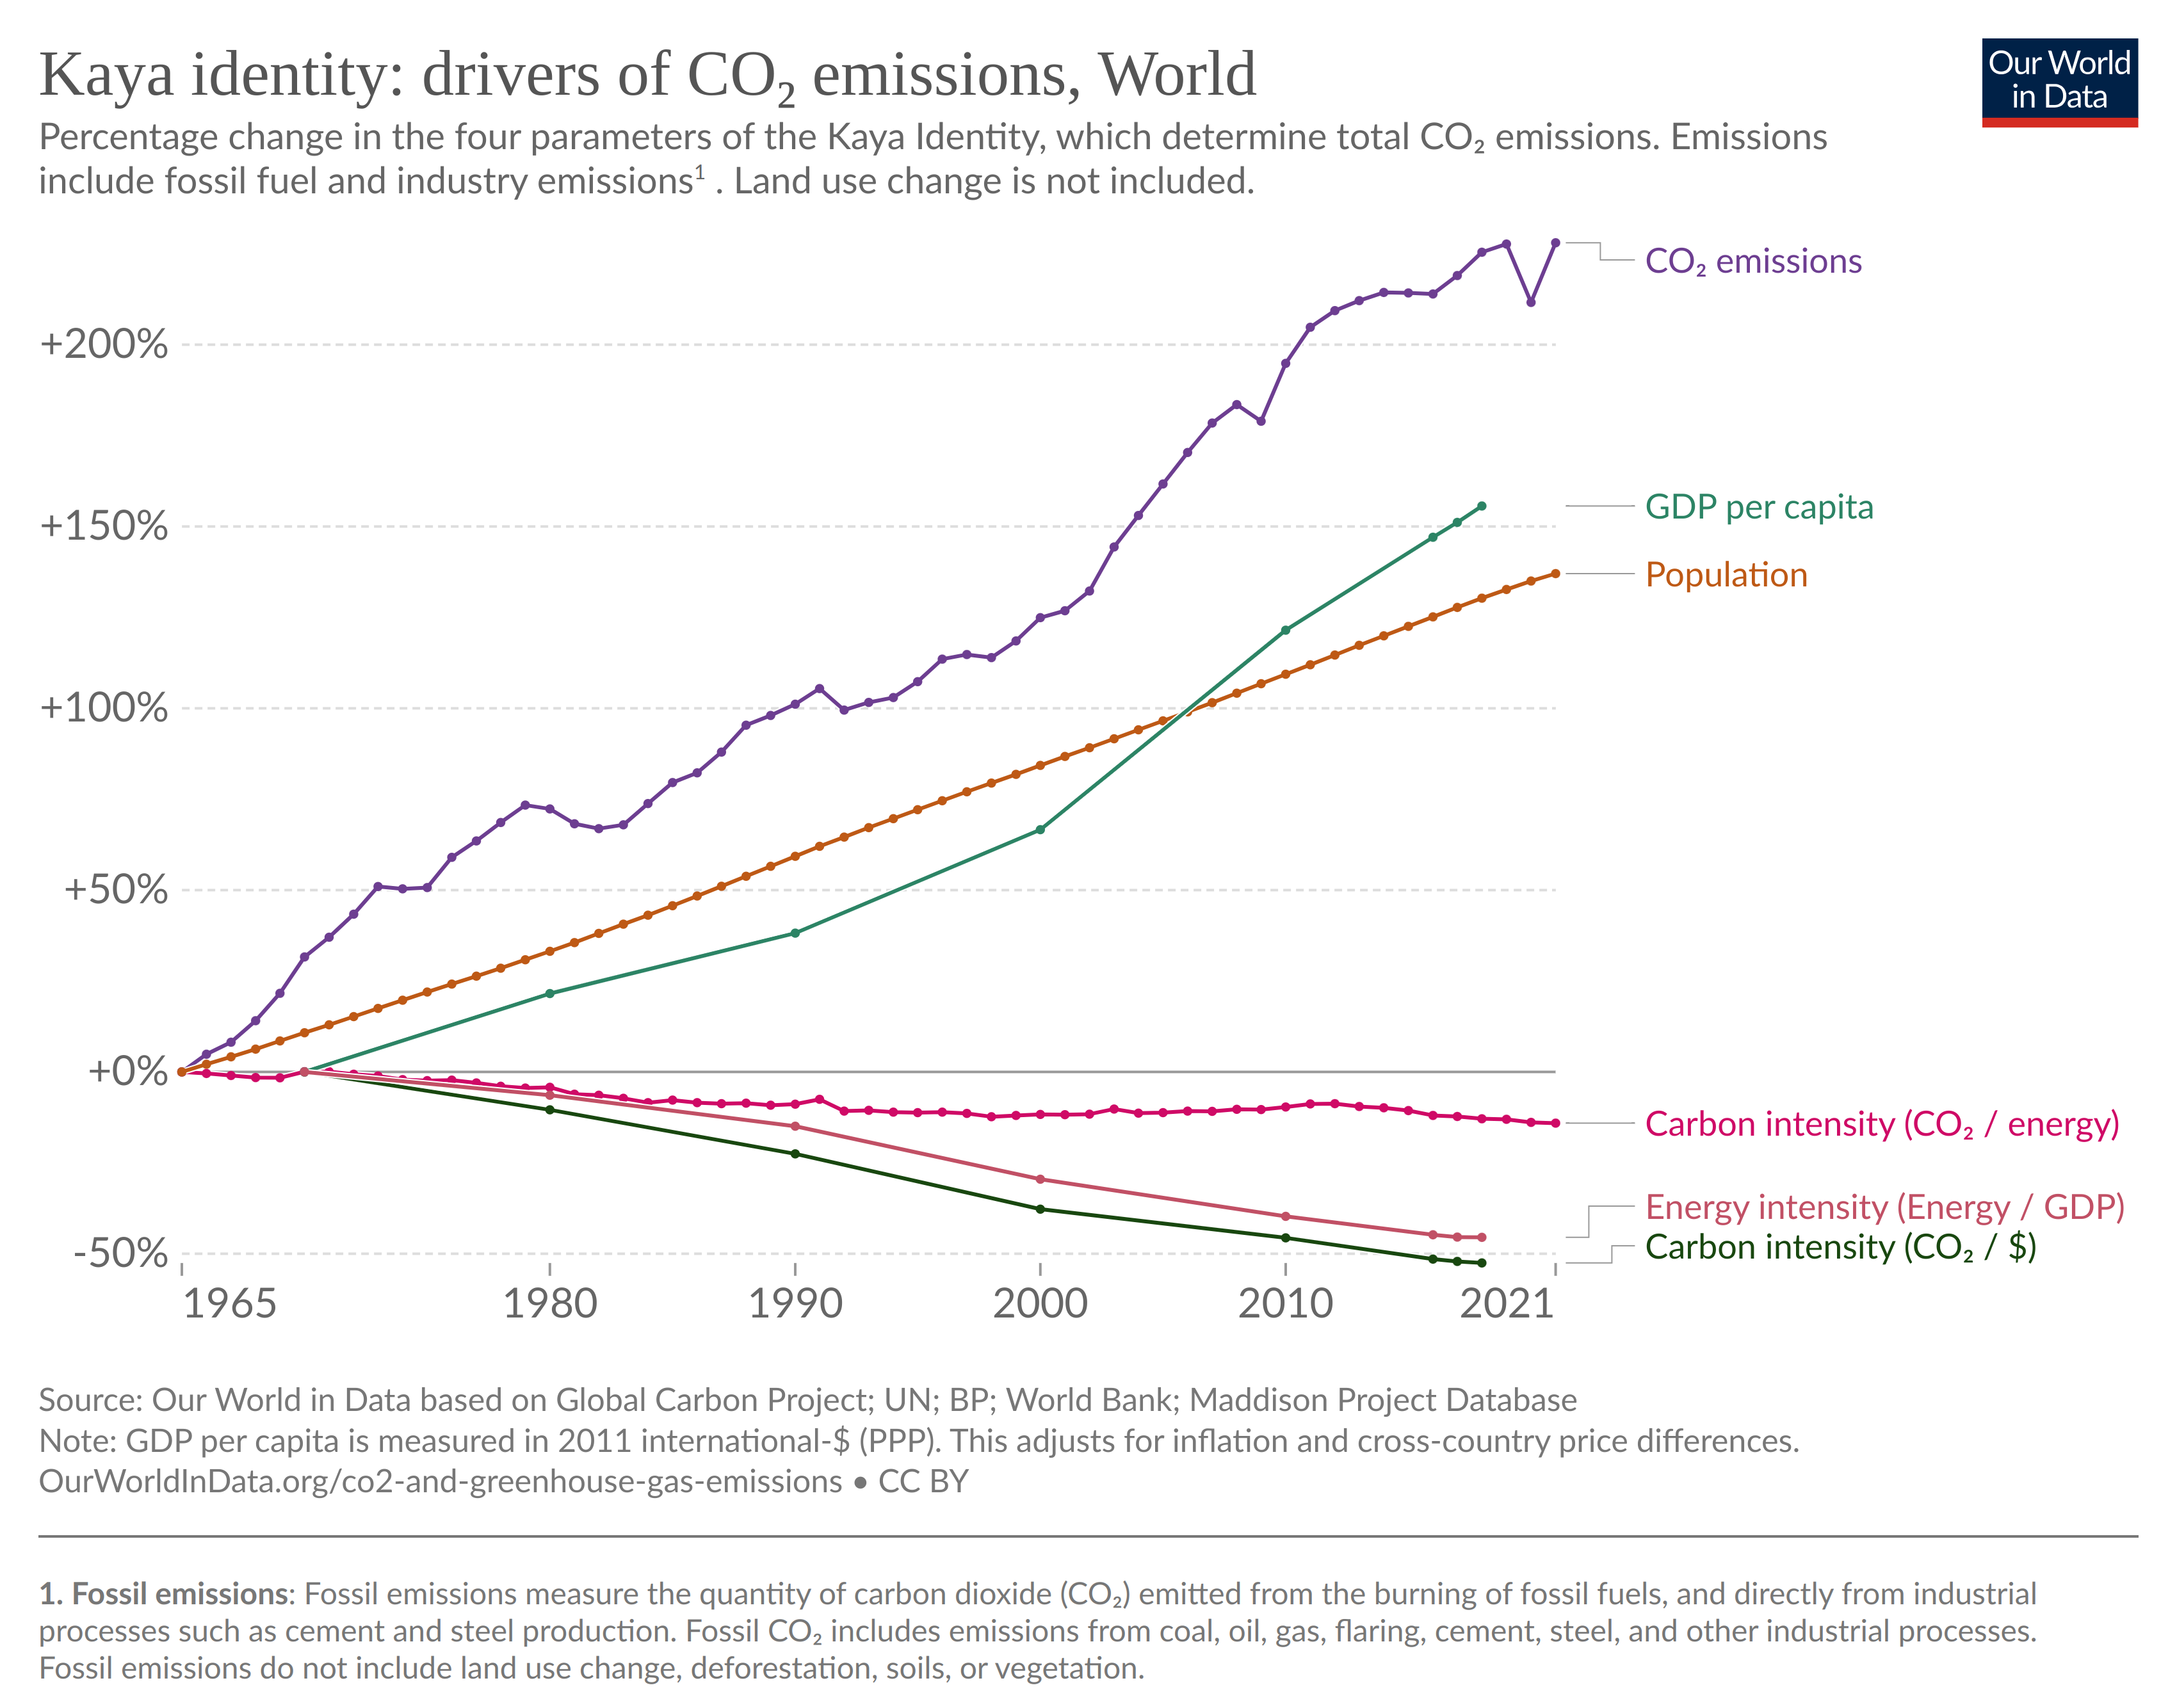
\includegraphics[width=0.55\textwidth]{figures/kaya-components.png}
    \caption{The Components of the Kaya Identity}
    \label{fig:kaya_components}
\end{figure}

\subsection{SSPs and RCPs}
\label{sec:ssps_rcps}

\textbf{Representative Concentration Pathways} (RCPs), are scenarios of future 
concentrations of greenhouse gases and other forcings. RCPs were used in the 
(\gls{IPCC}'s) Fifth Assessment Report.

The RCPs are named after their radiative forcing target level for the year 2100,
expressed in (W/m$^2$). There are four RCPs: 

\begin{itemize}
    \item \textbf{RCP 2.6}: This is a "peak and decline" scenario, where greenhouse gas
    emissions peak between 2010 and 2020, with substantial declines thereafter. By 
    2100, the additional radiative forcing is limited to 2.6 W/m$^2$.

    \item \textbf{RCP 4.5 and RCP 6}: These are stabilization scenarios where total radiative 
    forcing is stabilized before 2100 by applying a range of technologies and 
    strategies for reducing greenhouse gas emissions. The additional radiative 
    forcing in 2100 is 4.5 W/m$^2$ and 6 W/m$^2$, respectively.

    \item \textbf{RCP 8.5}: This is a rising radiative forcing pathway leading to 8.5 W/m$^2$ by 
    2100. This scenario assumes that emissions continue to rise throughout the 21st
    century.
\end{itemize}

These pathways provide inputs for climate model simulations to project future 
climate change. It's important to note that they're not predictions or forecasts,
but are plausible scenarios based on specific assumptions about future 
socio-economic development, technological changes, and policy interventions. 

The RPC approach has been extensively criticised by placing too much emphasis on
the most pessimistic of outcomes. As a result thereof, the \gls{IPCC} has
introduced a new set of scenarios for the Sixth Assessment Report, called the
\textbf{Shared Socioeconomic Pathways} (SSPs).\\


\noindent The SSPs link population growth and movement, technological development, energy
production and use, land use and cost to future greenhouse gas and aerosol
emissions into 5 different ``choices'' or scenarios that are as follows (directly
quoted):
\begin{itemize}
    \item \textbf{SSP1: Taking the Green Road}. World shifts towards a more sustainable
    path, common solutions to health and educational issues, economic growth
    places emphasis on human well-being. Greater equality results.
    \item \textbf{SSP2: Middle of the Road}. Social, economic and technological trends follow
    historical patterns leading to uneven growth. There is slow progress
    towards sustainable development goals.
    \item \textbf{SSP3: Regional Rivalry - A Rocky Road}. Nations put their own interests first
    at the expense of wider development and international action on sustainable
    development goals (e.g. health, education, climate).
    \item \textbf{SSP4: Inequality - A Road Divided}. Increasing inequality both across and
    within nations. Effectively the rich get richer and the poor get poorer.
    Conflict and unrest become increasingly common.
    \item \textbf{SSP5: Fossil-fuelled development - Taking the Highway}. Growth in innovation
    and competitive (but integrated) markets allows rapid technological progress.
    Strong investment in health and education. Development is fuelled by fossil
    fuel exploitation. Geo-engineering is a viable option (see section 
    \ref{sec:geoengineering})
\end{itemize}

The different SSPs lead to different emission levels (with SSP1 being the lowest
and SSP5 being the highest). Aerosol emissions are reduced in all SSPs.
It is important to note that none of these scenarios
are able to match the Paris Agreement goals without additional implementation of
mitigation strategies (carbon capture, geoengineering etc.).\\

For some lower-level details on the SSPs (GDP, GDP per capita, total energy 
demand, impact on the global mean surface temperature) see L12 slides 18 onwards or 
\href{https://www.sciencedirect.com/science/article/pii/S0959378016300681}{Riahi
\textit{et al.} 2017}.

